%=-=-=-=-=-=-=-=-=-=-=-=-=-=-=-=-=-=-=-=-=-=-=-=-=-=-=-=-=-=-=-=-=-=- CHAPTER 03
\chapter{Images, Figures \& Tables}

%=-=-=-=-=-=-=-=-=-=-=-=-=-=-=-=-=-=-=-=-=-=-=-=-=-=-=-=-=-=-=-=-=-=-=-= SECTION
\section{Storing Images}

Images can be easily included in your document by using the \cs{includegraphics}
command included with the graphics package. Before we include our first image, we 
should probably create a folder to hold all our images to keep our folder 
lean in terms of the number of files.  My personal preference is to keep all my 
images in the folder called \verb!~/assets!, which is relative to where the 
main file is located - the root of the project folder. If you are looking for 
a more refined organization of your images, then it is also possible to 
populate your assets folder with subfolders.

When we reference an image file, we need to provide both the path and file name.
Fortunately, there is a way to assign the path(s) where you store your images,
so you do not have to include the path to each image.  This can be done by 
including the \cs{graphicspath} command in the preamble of the script to assign
the path of where your images are stored.
\begin{dispListing}
\graphicspath{{/assets/}}
\end{dispListing}
It is also possible to define more than one path, which you might want to do 
if you are using subfolders to organize your images.  Just be careful to 
ensure all your images have unique names if you do decide to store your 
images in multiple folders.
\begin{dispListing}
\graphicspath{{/assets/images}{/assets/pdfs/}{/assets/matplotlib/}{/assets/tikz/}}
\end{dispListing}
This command will save you a lot of typing and frustration, so I would 
encourage you to try it.

%=-=-=-=-=-=-=-=-=-=-=-=-=-=-=-=-=-=-=-=-=-=-=-=-=-=-=-=-=-=-=-=-=-=-=-= SECTION
\section{Images}

To include an image into our document, we will use the \cs{includegraphics} 
command, which accepts the path and file name as its argument and can take 
on multiple options.  If you made use of the \cs{graphicspath} command made 
available by default for this template, then the argument is simplify the file 
name.  The file extension is optional, unless you have multiple files with the 
same name, but with different extensions. Yes, \verb!foo.pdf! are valid 
image files to include into your document. 
\begin{dispListing}
    \includegraphics{myimage.jpg}
    \includegraphics{myimage.pdf}
\end{dispListing}
The option that I set most often when using the \cs{includegraphics}
command is the width of the image.  For example, let's say that I want to 
include an image called \verb!image.pdf! into my document such that it is 
centered on the page and that the width of the image is set to a quarter of 
the text width of the page. 
\begin{dispExample}
\begin{center}
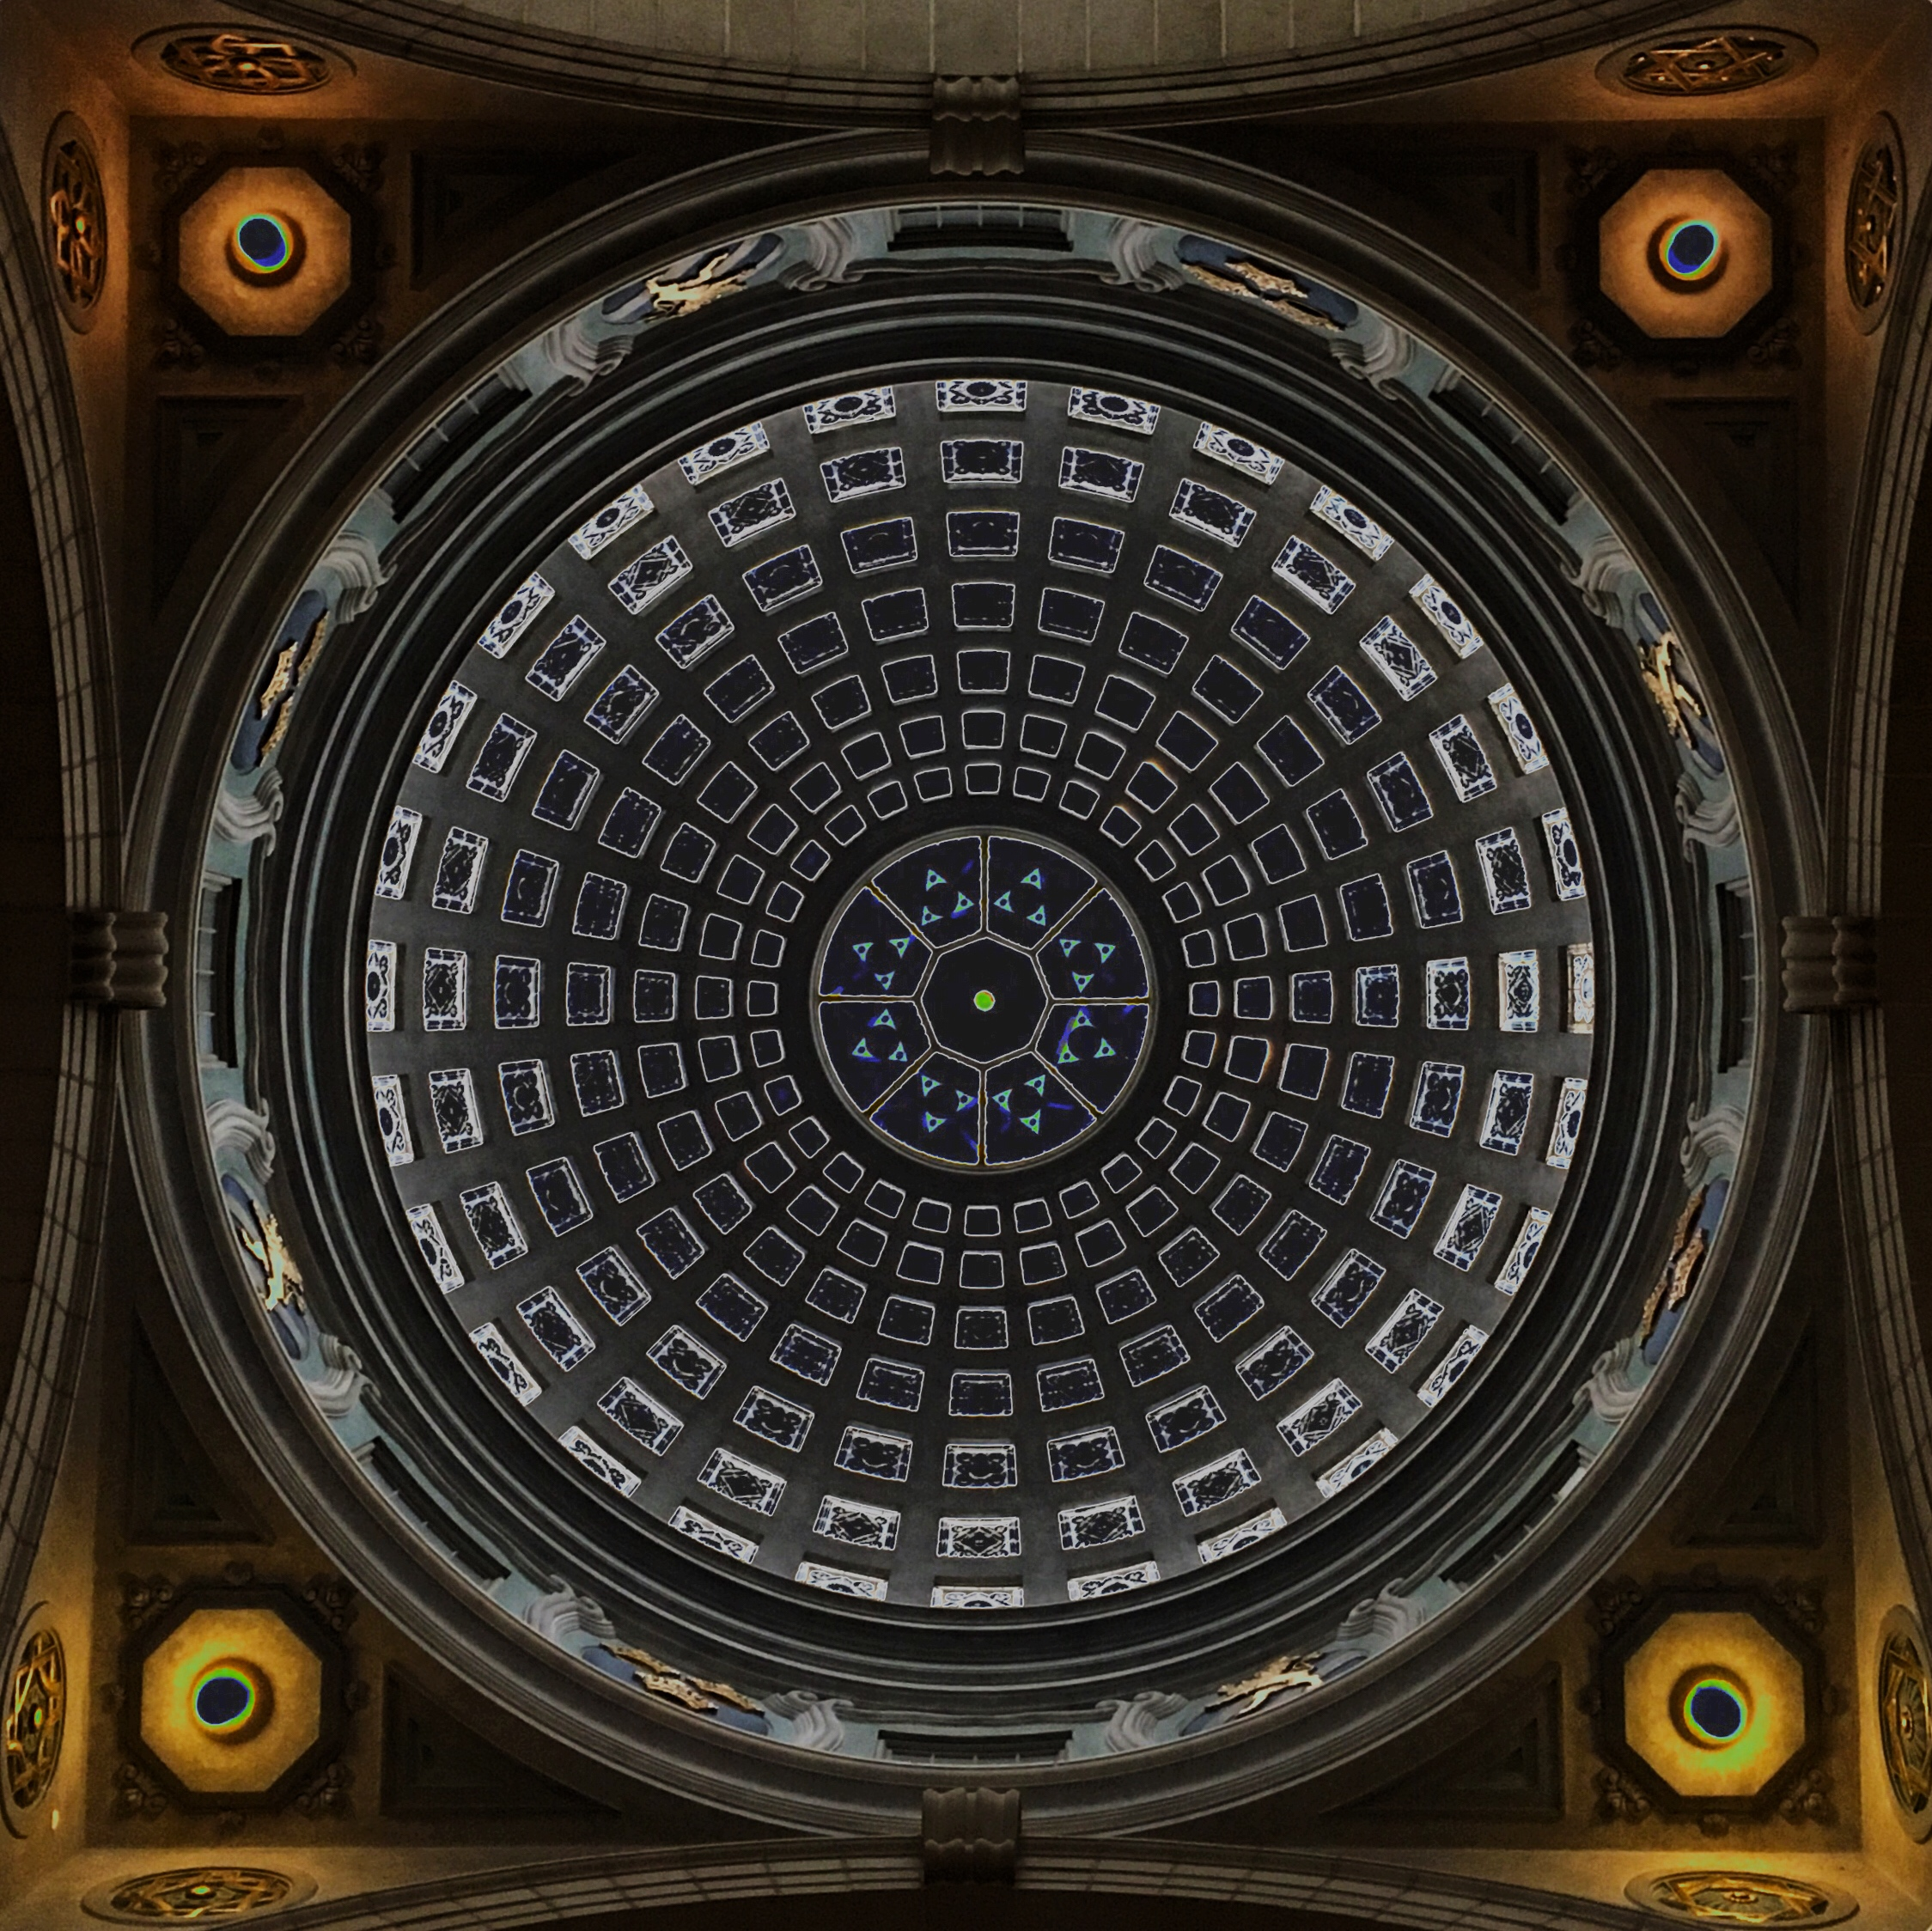
\includegraphics[width=0.25\textwidth]{image}
\end{center}
\end{dispExample}
Just be careful when working with raster images such as \verb!foo.jpg! as 
these types of images do not scale well.  I try to ensure that all my images 
are vector based such as a \verb!foo.pdf!, which allows for beautiful scaling.

% TODO Include height scale
% TODO Include scale
% TODO Include rotate 

%=-=-=-=-=-=-=-=-=-=-=-=-=-=-=-=-=-=-=-=-=-=-=-=-=-=-=-=-=-=-=-=-=-=-=-= SECTION
\section{Figures}

The \XeLaTeX\ engine is typesetting the document for us and placing images on 
the page is part of that process.  An inherent problem with images is that they 
cannot be broken across two pages like a paragraph of text.  A common
solution is to create a page break each time you have an image that spans over 
two pages.  Let's leave the typesetting to the engine because let's face it,
if you have many images that are spanning two pages, your document is not going 
to look good with all that extra whitespace created by forcing those page breaks.
The solution is a floating environment called a figure to embed your image. 

A float works by moving the image that does not fit on the page to a later one
and fill up the white space of the current page with text.  It is time to 
let go of implicitly referencing images by their placement of the document. 
We should now be referencing our images and let the engine calculate the best placement
of all our floats within our document.  It might feel better knowing that 
you can give your image a caption to provide some context as it might no 
longer be related to the surrounding text.  Just be ready for the engine to
never place the float where you would have placed it.

\begin{docEnvironment*}[doclang/environment content=includegraphics here]{figure}{\oarg{!htbp}}{}
\end{docEnvironment*}

You can see that the figure environment includes some optional arguments, called 
placement specifiers\cite{CTANPackageLshort}, that give you some control over where
the engine will place the float. The order in which the placement specifiers
are written is the priority the engine will give to placing your float within your 
documentation.  If no placement identifiers are given, then it will default to \oarg{tbp}. 
See table \cref{tbl:placementspecifiers} for a summary which each optional
argument does.
\begin{table}
\begin{tblr}{c X[l]}
\hline
\oarg{h} & Places the float \textbf{here} relative to the text you have written.
This should only be used for small floats. \\
\oarg{t} & Place the float at the \textbf{top} of the next available page.\\
\oarg{b} & Place the float at the \textbf{bottom} of the next available page. \\
\oarg{p} & Place on a \textbf{page} only containing floats. \\
\oarg{!} & Force one of the above options even if it does not look good.\\
\hline
\end{tblr}
\label{tbl:placementspecifiers}
\caption{Float Placement Specifiers}
\end{table}
You will probably want to reference your image at some point in your text and
will most likely want to give it a caption.  For this we are going to
use the figure environment, which will calculate the best position to place 
your image within the document.  Don't worry, there are ways to manually place 
the image where you would like it to appear.
\begin{docEnvironment}[doclang/environment content=image content goes here]{figure}{\oarg{h, t}}{}
    \begin{dispListing}
        \begin{center}
        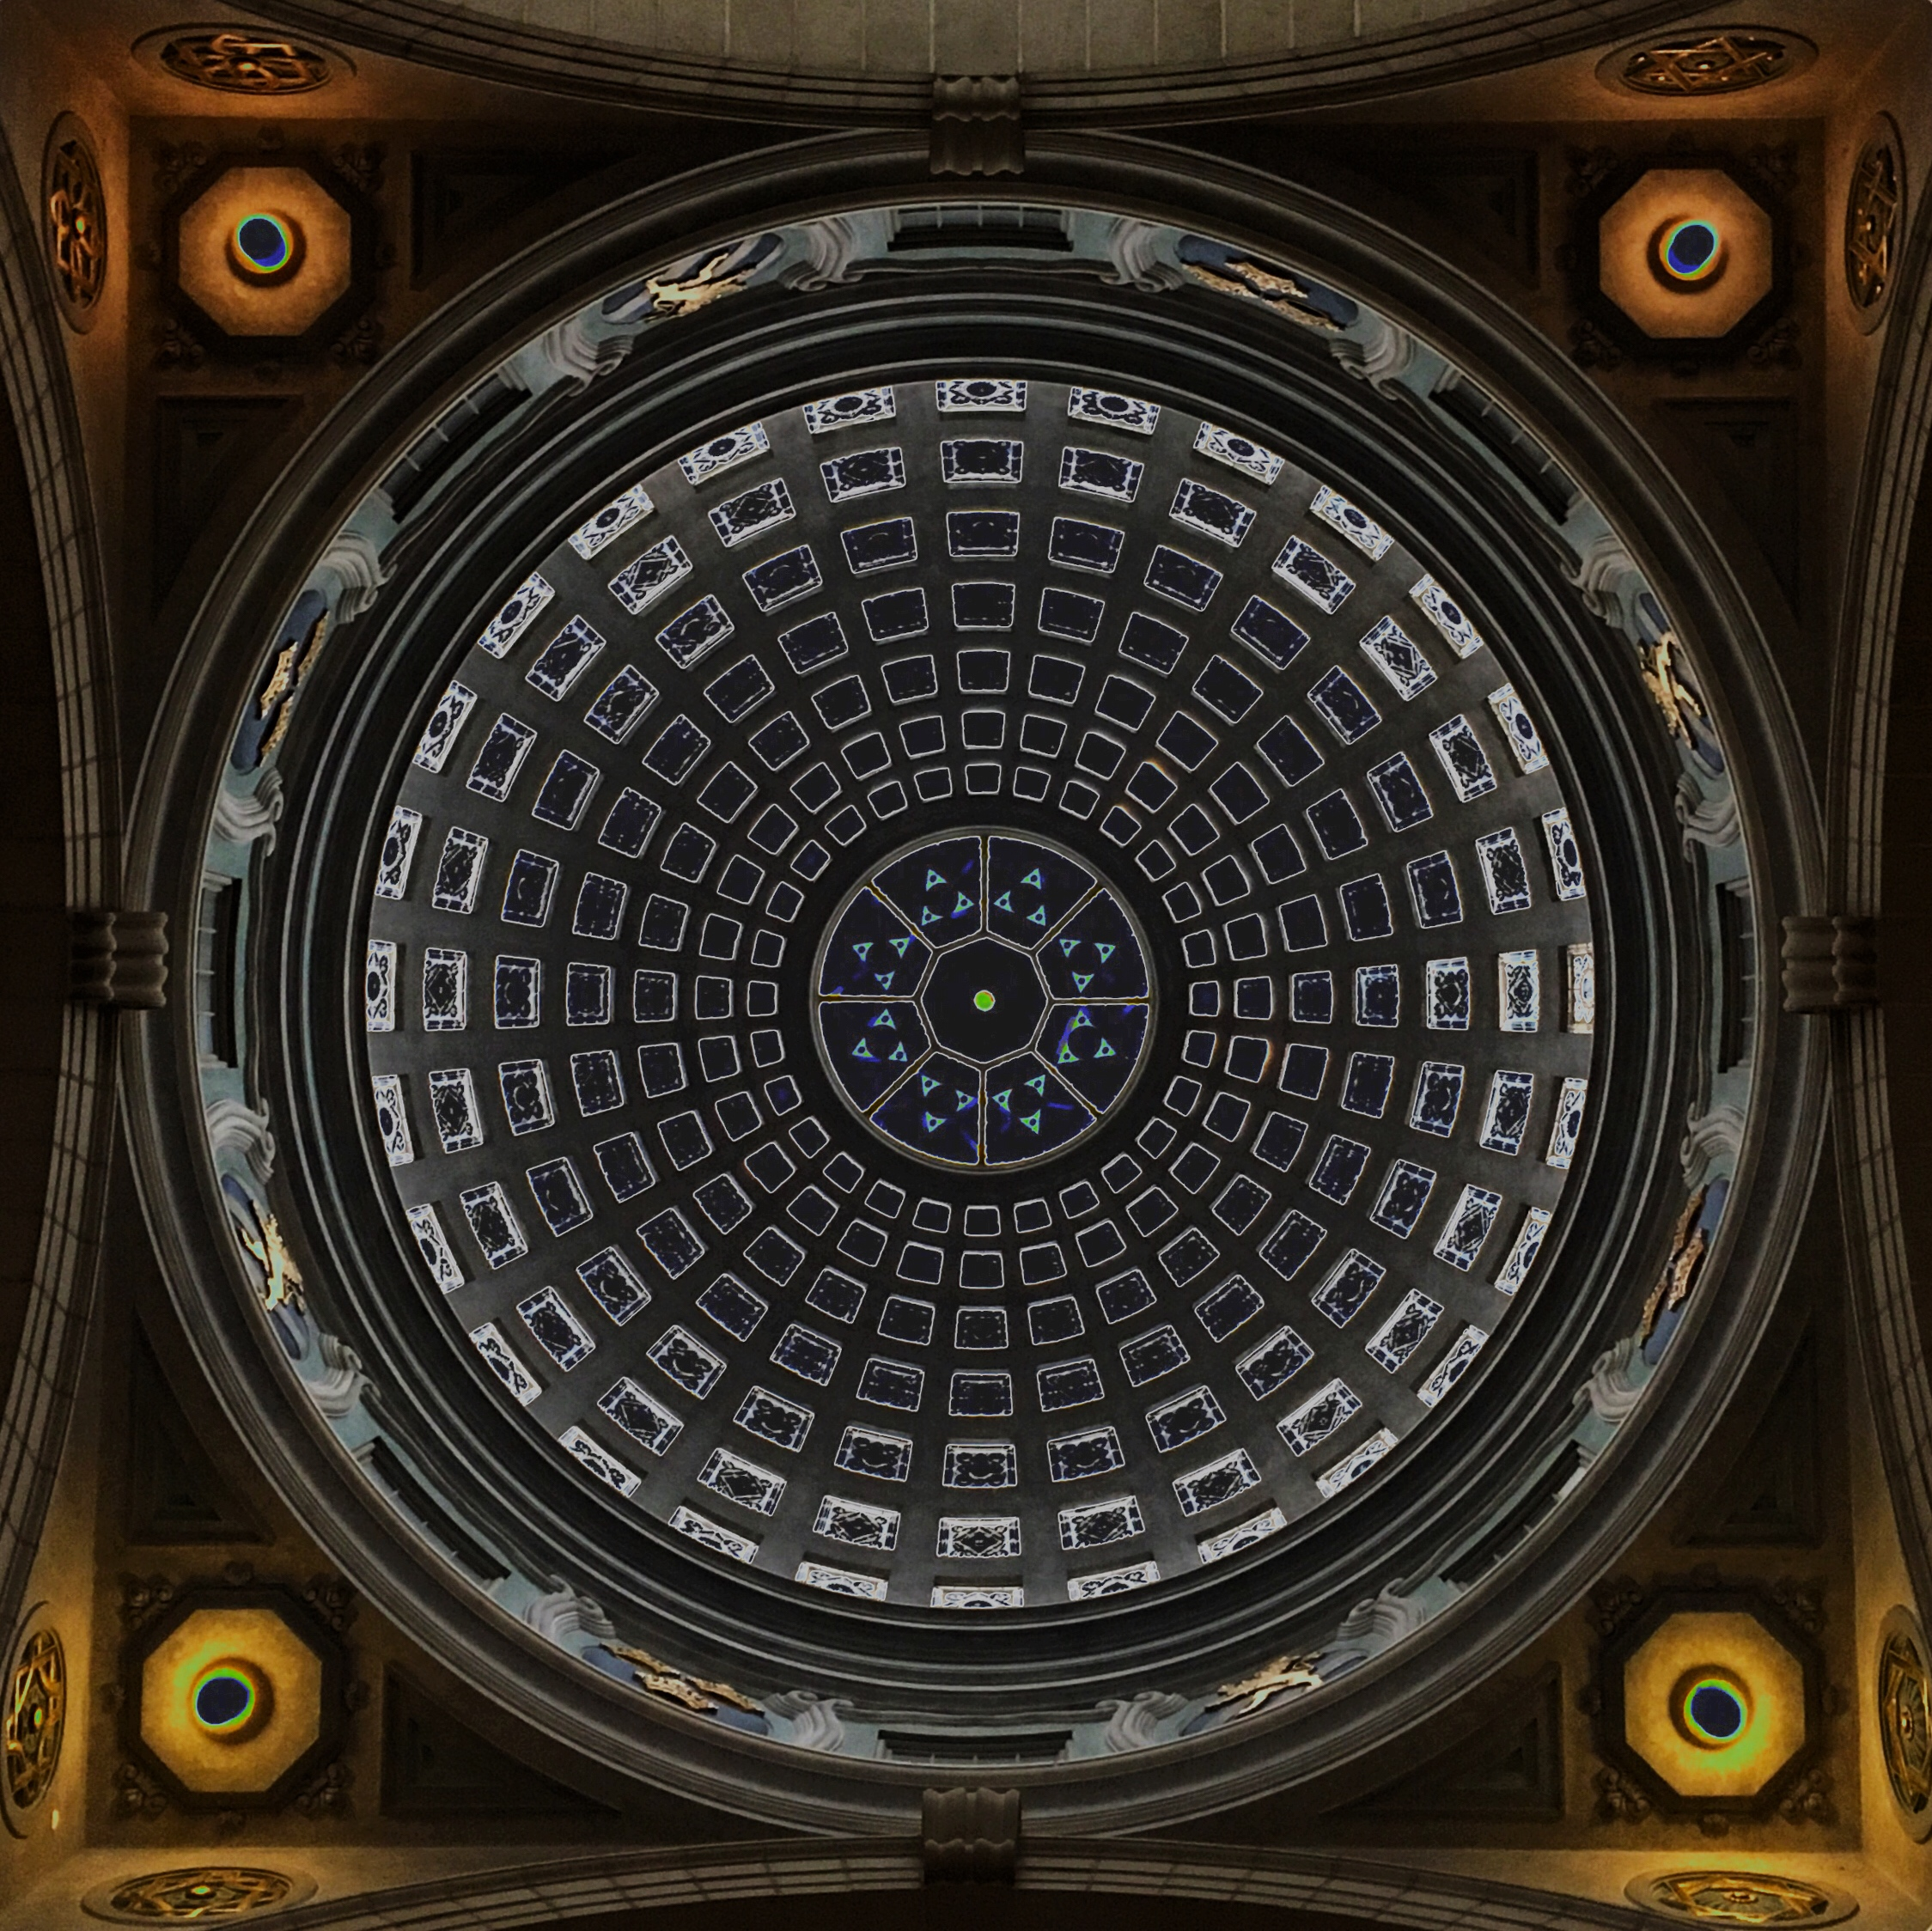
\includegraphics[width = 0.25\textwidth]{image.jpg}
        \end{center}
        \caption{Here is my excellent image.}
        \label{fig:img002}
        \end{dispListing}
\end{docEnvironment}
\begin{figure}[h]
    \begin{center}
    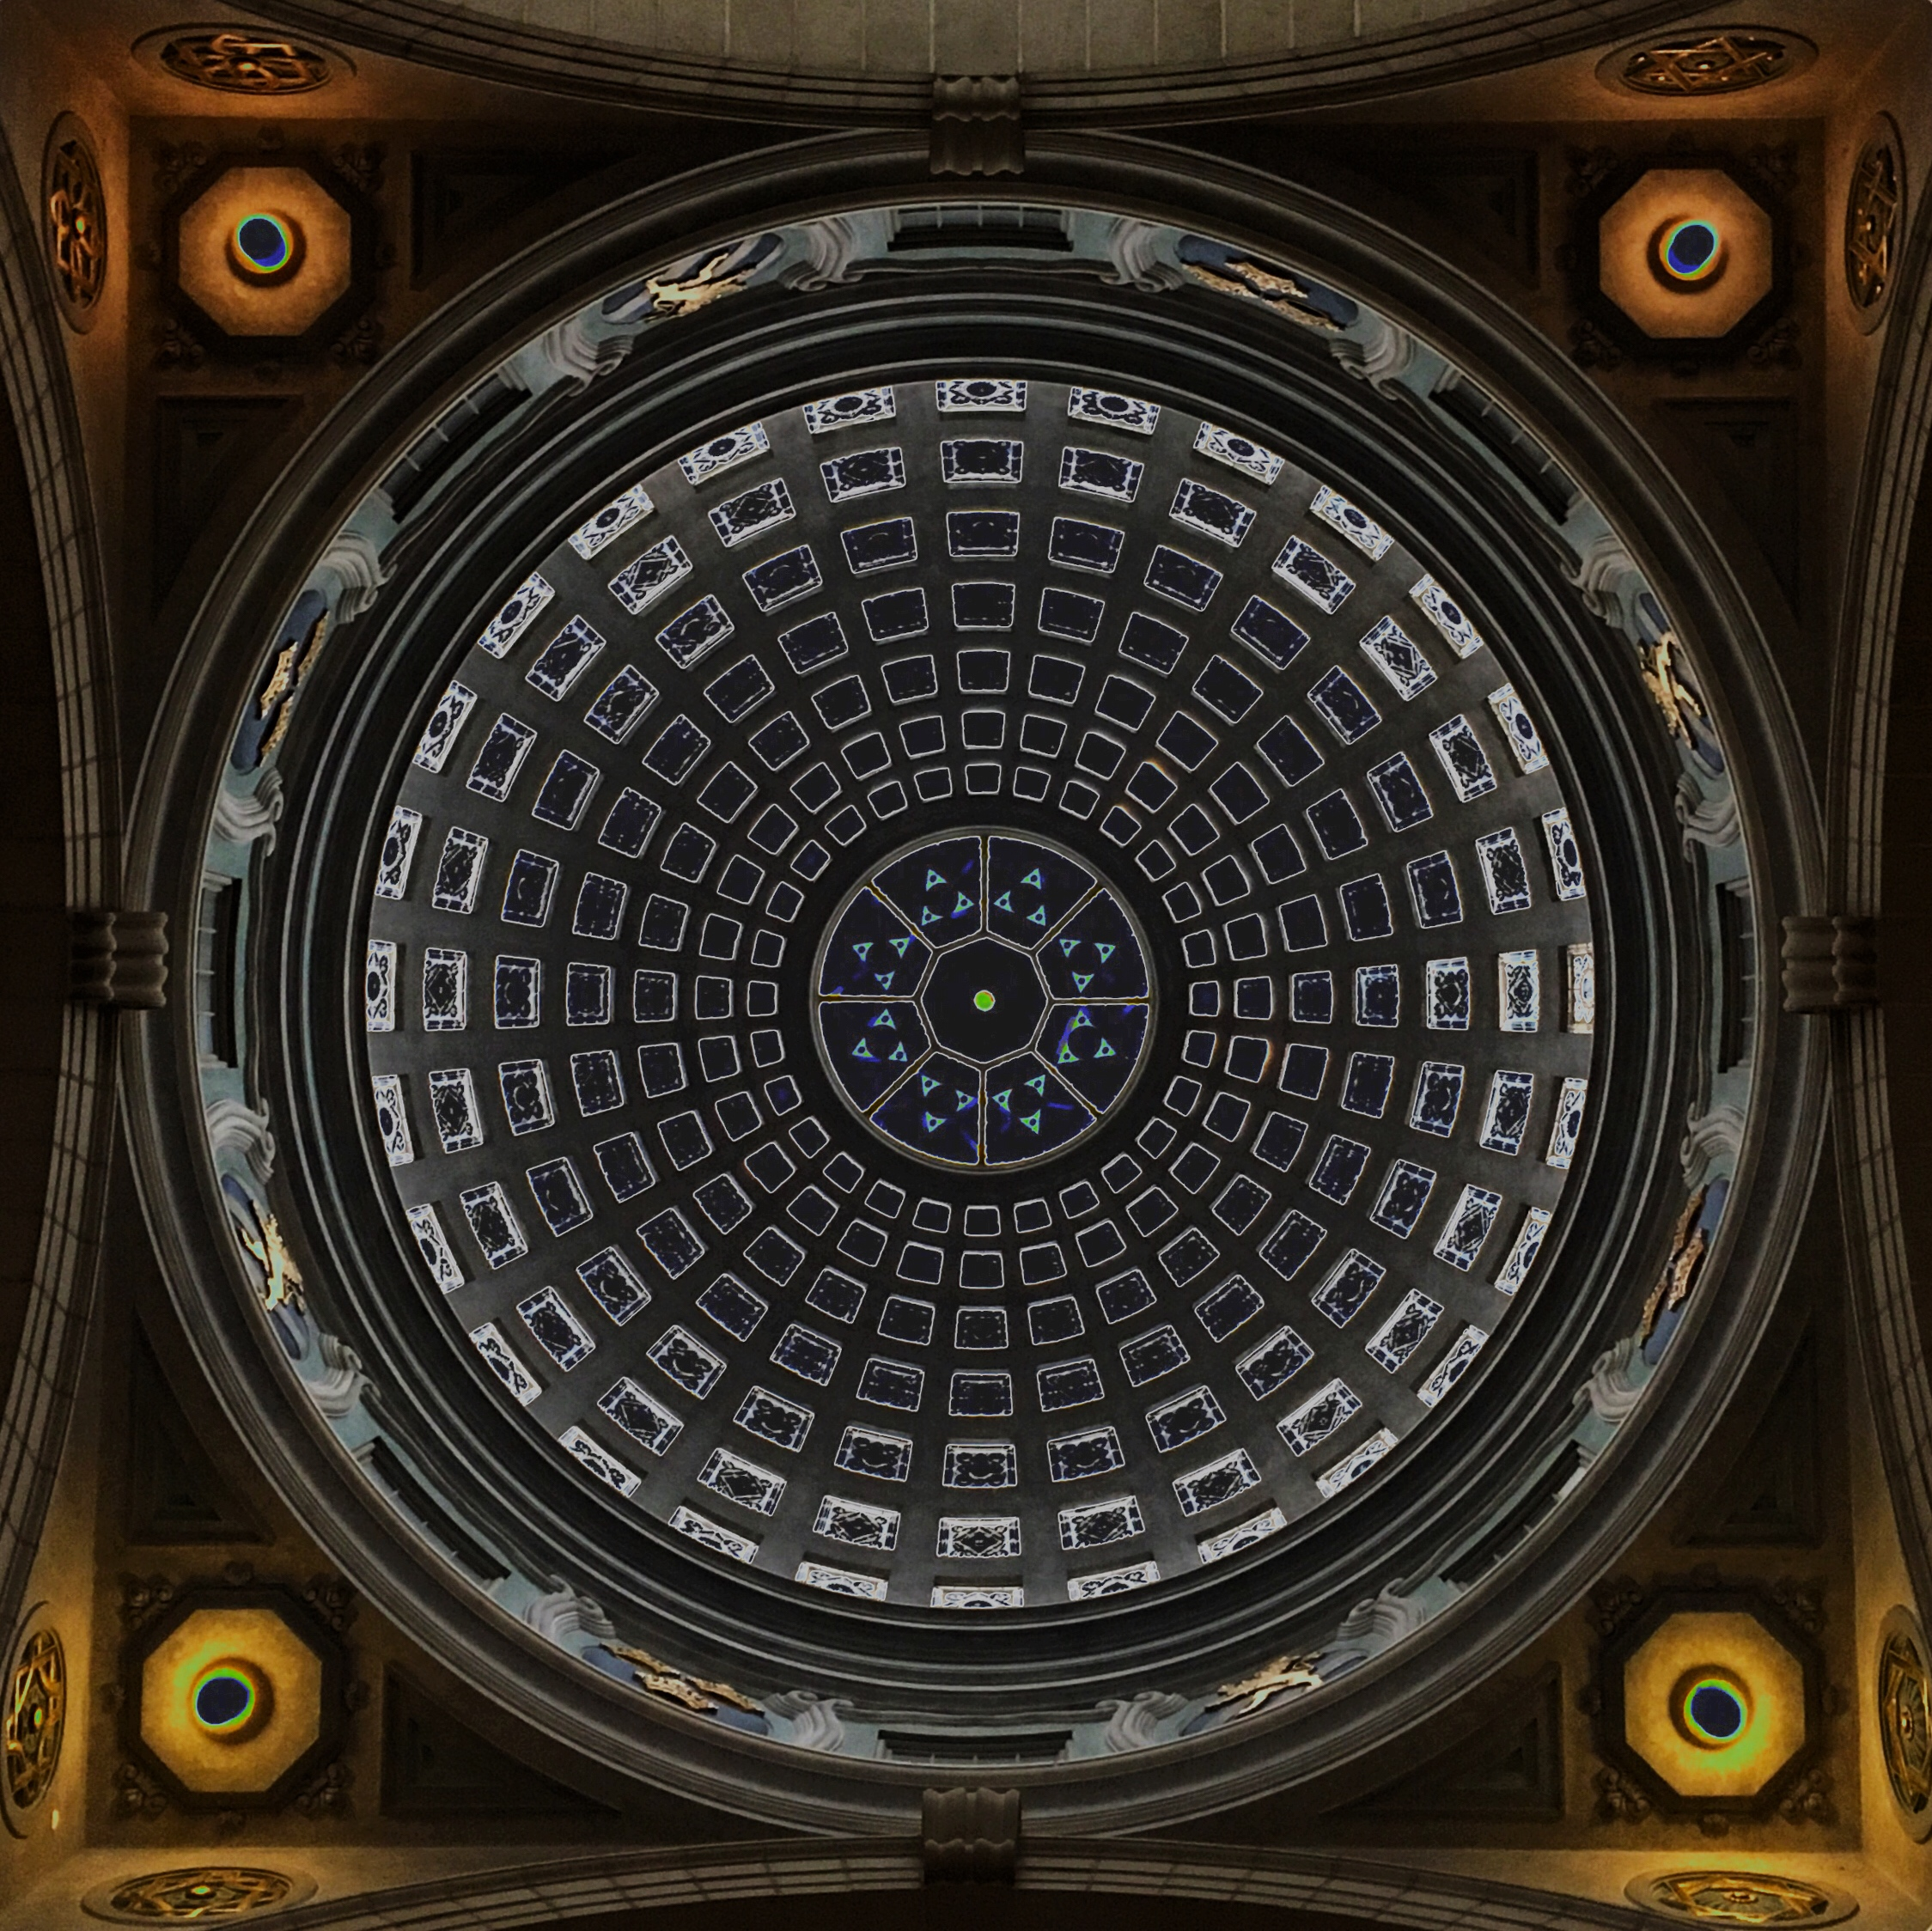
\includegraphics[width = 0.5\textwidth]{image.jpg}
    \end{center}
    \caption{Here is my excellent image.}
    \label{fig:img001}
\end{figure}
This would generate figure \ref{fig:img001}.

%=-=-=-=-=-=-=-=-=-=-=-=-=-=-=-=-=-=-=-=-=-=-=-=-=-=-=-=-=-=-=-=-=-=-=-= SECTION
\section{Multiple Horizontally Aligned Images}

Quite often it is the case that we want to include multiple horizontally
aligned images.  The figure environment is not well equipped for this task, so
we care going to make use of the subfigure package which will give us the 
subfigure environment that we can embed in our figure environment.  This will
enable us to assign both a caption and a label to each image separately.
\begin{docEnvironment}[doclang/environment content=image content goes here]{subfigure}{}{}
\begin{dispListing}
\begin{figure}
    \begin{center}
    \begin{subfigure}[b]{0.3\textwidth}
        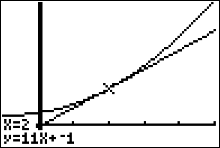
\includegraphics[width=\textwidth]{20170509-123642}
        \caption{Step 1}
        \label{fig:step1a}
    \end{subfigure}
    ~   % > > > Add desired spacing between images, e. g. ~, \quad, \qquad,
                % \hfill etc. (or a blank line to force the subfigure onto
                % a new line)
    \begin{subfigure}[b]{0.3\textwidth}
        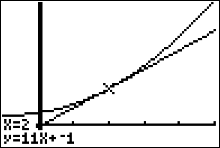
\includegraphics[width=\textwidth]{20170509-123642.png}
        \caption{Step 2}
        \label{fig:step2a}
    \end{subfigure}
    ~   % > > > Add desired spacing between images, e. g. ~, \quad, \qquad,
                % \hfill etc. (or a blank line to force the subfigure onto
                % a new line)
    \begin{subfigure}[b]{0.3\textwidth}
        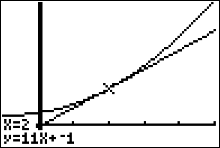
\includegraphics[width=\textwidth]{20170509-123642.png}
        \caption{Step 3}
        \label{fig:step3a}
    \end{subfigure}
    \caption{The Steps Shown}\label{fig:threestepsa}
    \end{center}
\end{figure}
\end{dispListing}
\end{docEnvironment}
\begin{figure}
    \begin{center}
    \begin{subfigure}[b]{0.3\textwidth}
        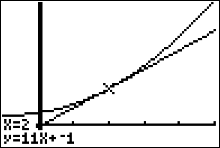
\includegraphics[width=\textwidth]{20170509-123642}
        \caption{Step 1}
        \label{fig:step1}
    \end{subfigure}
    ~   % > > > Add desired spacing between images, e. g. ~, \quad, \qquad,
                % \hfill etc. (or a blank line to force the subfigure onto
                % a new line)
    \begin{subfigure}[b]{0.3\textwidth}
        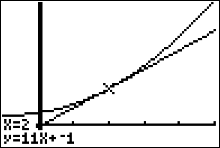
\includegraphics[width=\textwidth]{20170509-123642.png}
        \caption{Step 2}
        \label{fig:step2}
    \end{subfigure}
    ~   % > > > Add desired spacing between images, e. g. ~, \quad, \qquad,
                % \hfill etc. (or a blank line to force the subfigure onto
                % a new line)
    \begin{subfigure}[b]{0.3\textwidth}
        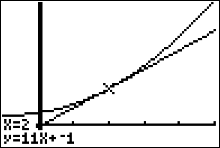
\includegraphics[width=\textwidth]{20170509-123642.png}
        \caption{Step 3}
        \label{fig:step3}
    \end{subfigure}
    \caption{The Steps Shown}\label{fig:threesteps}
    \end{center}
\end{figure}

%=-=-=-=-=-=-=-=-=-=-=-=-=-=-=-=-=-=-=-=-=-=-=-=-=-=-=-=-=-=-=-=-=-=-=-= SECTION
\section{Tables}

It is very likely that you will want to include tables in your document.  
Tables are not always easy to generate using \LaTeX ; however the tabularray 
package makes formatting tables a little easier then some of the more 
popular table packages such as tabularx.  Tabularray is well documented and
supports tables in both text and math modes.  The package and custom styles 
used for tables are included in the mhotables.sty custom package.  This makes 
it easy for you to use your favorite tables package by only having to modify
one line of code in the mhotext.sty.  Of course, by doing so this documentation 
document will no longer compile as it is dependent on mhotables.sty.

\begin{dispListing}
%\RequirePackage{mhotables.sty}
\RequirePackage{tabularx}
\end{dispListing}

The table itself is placed in a table environment, which will allow the 
\XeLaTeX\ engine to calculate the best place for the table within your
document very much the same way the figure environment works.  It will
also enable to give your table a descriptive label using the \cs{caption}
command and give it a label so that you can reference it in your document. 
I usually propend tbl: to my table captions to make them easier to look up.

\begin{dispListing}
\begin{table}
    \begin{center}
    \begin{tblr}
    % Code to format the table
    \end{tblr}
\end{center}
\label{tbl:myfirsttable}
\caption{This table will be included in the document soon.}
\end{table}
\end{dispListing}

\begin{dispExample}
\begin{center}
\(\begin{tblr}[ 
    caption = {These display fractions look awesome out of the box!},
    label = {tblr:fractions}
]{rrr}
\hline
\dfrac{2}{3} &  \dfrac{2}{3} &  \dfrac{1}{3} \\
\dfrac{2}{3} & -\dfrac{1}{3} & -\dfrac{2}{3} \\
\dfrac{1}{3} & -\dfrac{2}{3} &  \dfrac{2}{3} \\
\hline
\end{tblr} \)
\end{center}
\end{dispExample}

Another example in math mode, would be to make use of the \cs{diagbox}
command which has been enabled by including \cs{UseTblrLibrary{diagbox}}
in the preamble of the style file.  Don't worry this is included by 
default.

\begin{dispExample}
    \begin{center}
    \(\begin{tblr}{|c||c|c|c|c|c|c||}
    \hline
    \diagbox{f(x)}{x}   &   0   &   1   &   2   &   3   &   4   &   5\\
    \hline
    x^2                 &   0   &   \SetCell{bg=nordEleven,fg=nordFour} \smile  &   3   &   9   &   16  &   25 \\
    \hline
    \end{tblr} \)
    \end{center}
    \end{dispExample}

\begin{table}
    \caption{hello world}
    \begin{center}
    \(\begin{tblr}{|c||c|c|c|c|c|c|}
    \hline
    \diagbox{f(x)}{x}   &   \cpoint   &   \interval   &   2   &   3   &   4   &   5\\
    \hline
    x^2                 &   \cellTeal \checkcirc   &  \cellRed \decf &   \cellGrey \stationary  &   \cellGreen \incf   &   \cellTeal +  &   \cellOrange - \\
    \hline
    \end{tblr} \)
    \end{center}
\end{table}


%%% Local Variables:
%%% mode: latex
%%% TeX-master: "../main"
%%% End:
